% !TEX root = BA-Bericht.tex
\chapter{Einleitung}
\label{ch:Einleitung}

Das Internet Protokoll (IP) ist einer der wichtigsten Grundsteine für das heutige Internet.
Es wurde jedoch damals nicht unter den Gesichtspunkten wie Datenschutz, Privatsphäre und Sicherheit designt,
da es wohl eher darum, überhaupt ein Protokoll zu haben, um Nachrichten in einem Netzwerk verschicken und von Knoten zu Knoten weiterleiten zu können.
Mittlerweile gibt es jedoch verschiedene Anonymisierungsnetzwerke, welche in diesem Bereich Abhilfe schaffen könnten.
Eines davon nennt sich ``\glstext{i2p}'' (kurz \glsname{i2p}), welches in dieser Arbeit genauer untersucht wird.
Die Performanz von Anonymisierungsnetzwerken ist aber immer schlechter als die Performanz des Internet Protokolls (IP).
Denn einerseits verwenden die Anonymisierungsnetzwerke das Internet Protokoll (IP) als Basis und andererseits hat Anonymität in einem Netzwerk immer den Preis von höherer Netzwerkbandbreite oder höherer Latenz (siehe Abschnitt~\fullref{sec:anonymitytrilemma}).
Dementsprechend lässt die Performanz von Anonymisierungsnetzwerken für Benutzer oft zu wünschen übrig.
Auch sonst gibt es für normale Benutzer nicht wirklich Gründe, wieso solch ein Netzwerk eingesetzt werden sollte,
da es kaum Anwendungen gibt und für viele Privatsphäre nicht oberste Priorität hat.

\section{Aufgabe und Problemstellung}\label{sec:aufgabe}

Der Verein DIVA.EXCHANGE\footnote{Webauftritt: \url{https://diva.exchange}} entwickelt einen Softwareprototypen DIVA.
Der Softwareprototyp soll aufzeigen, dass es möglich ist, eine \glstext{fullydistributed}e Handelsplattform zu entwickeln,
die sowohl sicher ist, als auch die Privatsphäre der Benutzer schützt.
Benutzer sollen digitale Werte austauschen können, ohne sich dabei zu kennen und ohne sich gegenseitig vertrauen zu müssen.
Es handelt sich hierbei um ein freies Softwareprojekt\footnote{Was ist ``freie Software''? Siehe \url{https://www.gnu.org/philosophy/free-sw.de.html}}.

Der Softwareprototyp besteht aus drei Schichten.
Die Handelsplattform und die dazugehörige Verwaltungssoftware stellen die oberste Schicht dar.
Darunter befindet sich eine Datenhaltungs- und Speicherschicht, basierend auf einer im Haus entwickelten Blockchain namens Divachain.
Auf der untersten Ebene, der Netzwerkschicht, wird \glsname{i2p} verwendet.
\glsname{i2p} soll die Basis bieten für den Softwareprototypen, um von Grund auf Anonymität und Sicherheit der Kommunikation sicherzustellen (siehe Abbildung~\fullref{fig:divax_overview}).

\begin{figure}[thp!]
    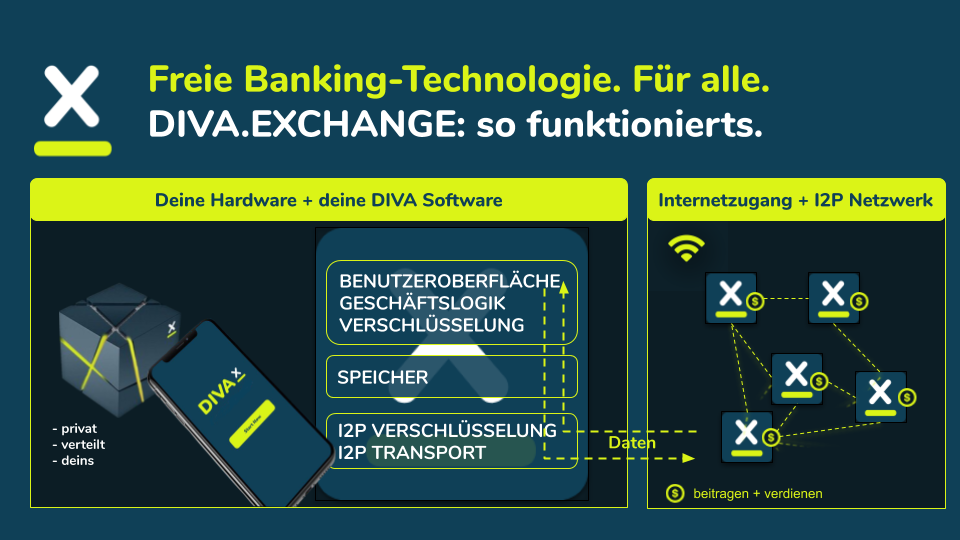
\includegraphics[width=1.0\textwidth]{img/divax-overview.png}
    \caption{Übersicht DIVA.EXCHANGE}\label{fig:divax_overview}
\end{figure}

Es besteht die Annahme, dass die Performanz des \glsname{i2p}-Netzwerks nicht ausreichend ist, um für Endbenutzer schnell reagierende Applikationen auf dem Netzwerk anbieten zu können.
Das Netzwerk ist verglichen mit dem \glsname{tor}-Netzwerk klein und es können grössere Latenzen entstehen, um Anonymität für die Netzwerkteilnehmer zu bieten.
Kurz vor Beginn dieser Arbeit dauerte das Hin- und Zurücksenden einer Nachricht durch das \glsname{i2p}-Netzwerk (Roundtrip) etwa drei bis acht Sekunden. Dies hat mehrere Gründe:

\begin{itemize}
    \item Eine Nachricht wird über mehrere Hops versendet und wird mehrmals weitergeleitet bevor sie beim Empfänger ankommt.
    \item Fallen Hops, aus müssen die Nachrichten über eine andere Route neu übermittelt werden.
    \item Jede Nachricht ist mehrfach verschlüsselt und jeder Knoten muss jeweils eine Verschlüsselungsschicht beim Weiterleiten einer Nachricht entfernen, was viele CPU-Zyklen kostet.
\end{itemize}
\\
Im Rahmen dieser Arbeit soll folgende Problemstellung untersucht werden:

\begin{hyp}[H\ref{hyp:first}] \label{hyp:first}
    Ist eine steigende Anzahl von I2P-Knoten für die I2P-Netzwerk-Latenz (tiefer) vorteilhaft?
    Können Nachrichten schneller vom Sender zum Empfänger gelangen je mehr Knoten das I2P-Netzwerk hat?
\end{hyp}

Damit Applikationen auf dem I2P-Netzwerk gut funktionieren, soll ermittelt werden, wie die Performanz
verbessert werden kann.
Siehe auch die komplette Aufgabenstellung, die im Anhang~\fullref{ch:aufgabenstellung} zu finden ist.

\section{Ziel und Vision}\label{sec:ziel}

Ziel ist es, aufzuzeigen, unter welchen Umständen und Rahmenbedingungen Anwendungen auf dem \glsname{i2p}-Netzwerk kürzere Latenzzeiten aufweisen
und somit aus Sicht eines Endbenutzers schneller reagieren.
Das Niveau an Anonymität soll aber zum Schutz der Privatsphäre nicht eingeschränkt werden.
Wird festgestellt, dass mehr Knoten in einem I2P-Netzwerk die Latenz verringern,
könnte es unter Umständen mehr Personen dazu bewegen selber \glsname{i2p}-Knoten zu betreiben.
Dies wiederum würde das Netzwerk stärken und diverse Netzwerkeffekte könnten auftreten.
Zum Beispiel könnte dies dazu führen, das mehr Entwickler Applikationen für das Netzwerk erstellen und es auch aus Benutzersicht attraktiver wird.

% Welche Ziele, Fragestellungen werden mit dem Projekt verfolgt? Die Bedeutung, Auswirkung und
% Relevanz dieses Projektes für die unterschiedlichen Beteiligten soll aufgeführt werden.
% Typischerweise wird hier ein Verweis auf die Aufgabenstellung im Anhang gemacht.
